\chapter{Исследовательская часть}

Технические характеристики устройства:
\begin{itemize}
    \item процессор: Intel(R) Core(TM) i5-10300H с тактовой частотой 2500000000 герц;
	\item ядра:	4;
	\item логические процессоры:	8;
    \item оперативная система: Windows 10;
    \item оперативная память: 8 ГБ.
\end{itemize}



\section{Анализ времени загрузки сцены в зависимости от количества подсолнухов}

\begin{table}[h!]
\centering
\caption{Время загрузки сцены в зависимости от количества подсолнухов}
\label{tab:sunflower_loading_time}
\begin{tabular}{|c|c|}
\hline
\textbf{Количество подсолнухов} & \textbf{Время загрузки (мс)} \\ \hline
1 & 118.23 \\ \hline
21 & 229.69 \\ \hline
41 & 471.19 \\ \hline
61 & 760.25 \\ \hline
81 & 1201.38 \\ \hline
101 & 1101.29 \\ \hline
121 & 1269.22 \\ \hline
141 & 1907.86 \\ \hline
161 & 2139.81 \\ \hline
181 & 2201.83 \\ \hline
201 & 2376.41 \\ \hline
221 & 2935.29 \\ \hline
241 & 2769.19 \\ \hline
261 & 2993.32 \\ \hline
281 & 3676.13 \\ \hline
301 & 3488.16 \\ \hline
321 & 3478.32 \\ \hline
341 & 3964.03 \\ \hline
361 & 4107.77 \\ \hline
381 & 4485.53 \\ \hline
401 & 4510.49 \\ \hline
\end{tabular}
\end{table}

На рисункe~\ref{images:graph_1} представлен график времени загрузки сцены в зависимости от количества подсолнухов.
\begin{figure}[H]
    \centering
    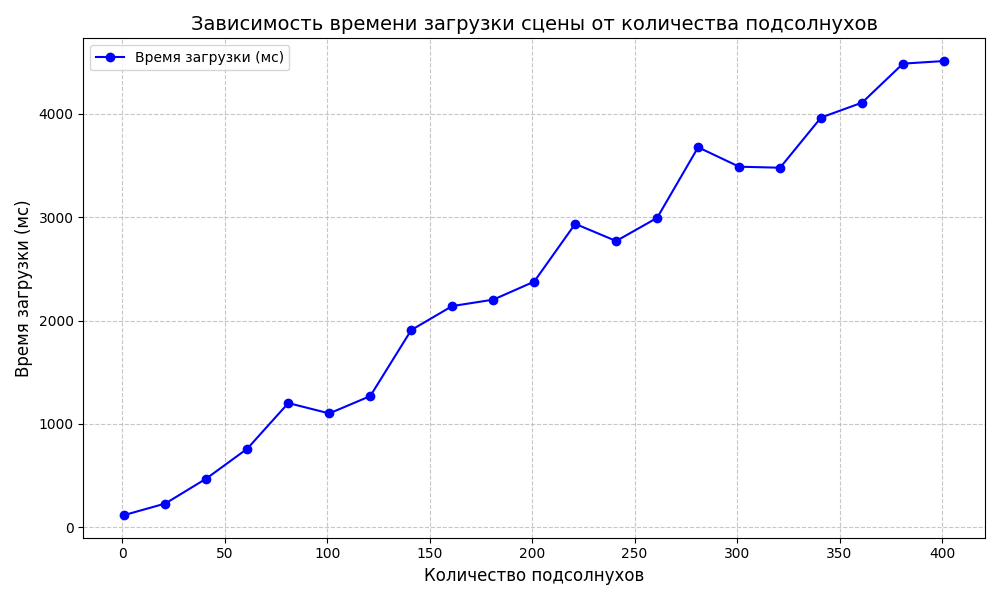
\includegraphics[width=155mm]{images/graph_1}
    \caption{График времени загрузки сцены в зависимости от количества подсолнухов.}
    \label{images:graph_1}
\end{figure}

\subsection{Общая тенденция}
\begin{itemize}
    \item Время загрузки увеличивается с ростом количества подсолнухов. Это ожидаемо, так как больше объектов требуют больше ресурсов для создания и рендеринга.
\end{itemize}

\subsection{Локальные колебания}
\begin{itemize}
    \item В некоторых случаях время загрузки может немного уменьшаться (например, для 101 подсолнуха время меньше, чем для 81). Это может быть связано с тем, что каждая модель подсолнуха имеет случайные характеристики.
\end{itemize}

\subsection{Вывод}
\begin{itemize}
    \item Данные показывают, что время загрузки увеличивается с ростом количества подсолнухов, но могут наблюдаться локальные колебания из-за случайных факторов.
\end{itemize}


\section{Анализ времени загрузки сцены в зависимости от размеров сцены}

\begin{table}[h!]
\centering
\caption{Время загрузки сцены (в мс) при различных размерах сцены}
\label{tab:scene_loading_time}
\begin{tabular}{|c|*{11}{c|}} % Исправлено количество столбцов
\hline
\textbf{Ширина} & \textbf{10} & \textbf{210} & \textbf{410} & \textbf{610} & \textbf{810} & \textbf{1010} & \textbf{1210} & \textbf{1410} & \textbf{1610} & \textbf{1810} & \textbf{2010} \\ \hline
\textbf{10} & 732 & 600 & 616 & 588 & 520 & 606 & 567 & 515 & 577 & 685 & 579 \\ \hline
\textbf{210} & 545 & 541 & 596 & 601 & 556 & 577 & 833 & 551 & 556 & 708 & 523 \\ \hline % Исправлено
\textbf{410} & 666 & 536 & 625 & 511 & 549 & 533 & 556 & 592 & 780 & 505 & 682 \\ \hline
\textbf{610} & 532 & 679 & 569 & 548 & 586 & 513 & 518 & 542 & 515 & 542 & 569 \\ \hline
\textbf{810} & 508 & 556 & 538 & 535 & 509 & 549 & 534 & 548 & 561 & 520 & 566 \\ \hline
\textbf{1010} & 527 & 539 & 534 & 530 & 500 & 565 & 562 & 551 & 524 & 534 & 543 \\ \hline
\textbf{1210} & 590 & 600 & 520 & 516 & 514 & 527 & 531 & 543 & 543 & 507 & 499 \\ \hline
\textbf{1410} & 601 & 645 & 527 & 542 & 533 & 528 & 512 & 612 & 556 & 723 & 529 \\ \hline
\textbf{1610} & 566 & 548 & 570 & 525 & 496 & 877 & 788 & 782 & 536 & 530 & 536 \\ \hline
\textbf{1810} & 544 & 515 & 595 & 526 & 537 & 522 & 589 & 541 & 538 & 561 & 545 \\ \hline
\textbf{2010} & 490 & 539 & 669 & 690 & 560 & 565 & 527 & 531 & 502 & 572 & 552 \\ \hline
\end{tabular}
\end{table}

На рисункe~\ref{images:graph_3} представлена тепловая карта времени загрузки сцены в зависимости от её ширины и высоты.
\begin{figure}[H]
    \centering
    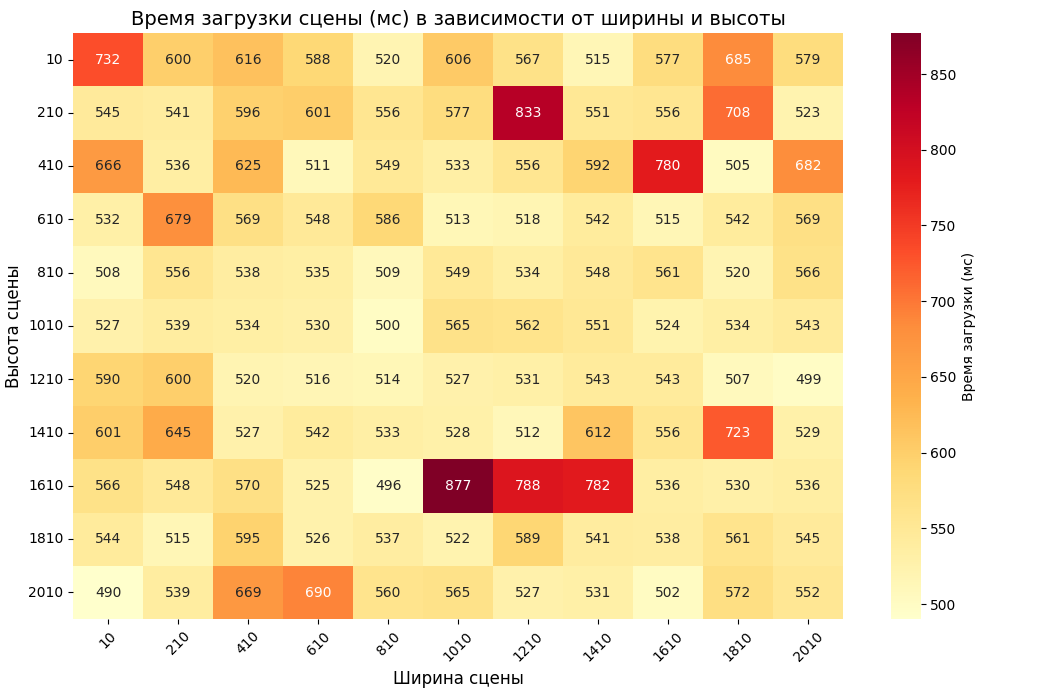
\includegraphics[width=155mm]{images/graph_3}
    \caption{Тепловая карта времени загрузки сцены в зависимости от её ширины и высоты.}
    \label{images:graph_3}
\end{figure}


\subsection{Общая тенденция}
\begin{itemize}
    \item Время загрузки сцены варьируется в диапазоне от \textbf{489,74 мс} до \textbf{877,27 мс}.
    \item Наблюдается отсутствие явной линейной зависимости между размером сцены (шириной и длиной) и временем загрузки.
\end{itemize}

\subsection{Зависимость от ширины и длины}
\begin{itemize}
    \item \textbf{Ширина сцены}:
    \begin{itemize}
        \item для ширины 10 время загрузки варьируется от 515,48 мс до 731,87 мс;
        \item для ширины 2010 время загрузки варьируется от 489,74 мс до 689,58 мс;
        \item нет явной закономерности, что увеличение ширины приводит к увеличению времени загрузки.
    \end{itemize}
    
    \item \textbf{Длина сцены}:
    \begin{itemize}
        \item для длины 10 время загрузки варьируется от 489,74 мс до 731,87 мс;
        \item для длины 2010 время загрузки варьируется от 498,59 мс до 684,53 мс;
        \item аналогично, увеличение длины не всегда приводит к увеличению времени загрузки.
    \end{itemize}
\end{itemize}

\subsection{Аномальные значения}
\begin{itemize}
    \item Наблюдаются выбросы в данных:
    \begin{itemize}
        \item \textbf{877,27 мс} (ширина: 1610, длина: 1010).
        \item \textbf{833,34 мс} (ширина: 210, длина: 1210).
        \item \textbf{781,50 мс} (ширина: 1610, длина: 1410).
    \end{itemize}
    
    \item Эти значения могут быть связаны с различными причинами, такими как:
    \begin{itemize}
        \item пиковая нагрузка на систему в момент загрузки;
        \item особенности рендеринга для определённых размеров сцены;
        \item фоновые процессы, которые могли повлиять на замеры.
    \end{itemize}
\end{itemize}

\subsection{Стабильность времени загрузки}
\begin{itemize}
    \item Для большинства сочетаний ширины и длины время загрузки находится в диапазоне 500–600 мс.
    \item Это указывает на стабильную производительность системы при изменении размеров сцены.
\end{itemize}

\subsection{Вывод}
\begin{itemize}
    \item Данные показывают, что время загрузки сцены с 50 подсолнухами не зависит напрямую от размеров сцены.
    \item Наблюдаются локальные колебания, которые могут быть связаны с особенностями работы системы или случайными факторами.
\end{itemize}


\section{Анализ загруженностьи процессора в зависимости от количества подсолнухов}

\begin{table}[h!]
\centering
\caption{Загруженность процессора в зависимости от количества подсолнухов}
\label{tab:cpu_usage}
\begin{tabular}{|c|c|}
\hline
\textbf{Количество подсолнухов} & \textbf{Загруженность процессора (\%)} \\ \hline
1 & 2,73 \\ \hline
21 & 2,23 \\ \hline
41 & 1,49 \\ \hline
61 & 1,92 \\ \hline
81 & 1,50 \\ \hline
101 & 2,28 \\ \hline
121 & 1,98 \\ \hline
141 & 2,14 \\ \hline
161 & 1,36 \\ \hline
181 & 4,98 \\ \hline
201 & 2,98 \\ \hline
221 & 2,33 \\ \hline
241 & 2,04 \\ \hline
261 & 4,19 \\ \hline
281 & 3,02 \\ \hline
301 & 2,27 \\ \hline
321 & 1,60 \\ \hline
341 & 1,96 \\ \hline
361 & 1,89 \\ \hline
381 & 3,06 \\ \hline
401 & 4,48 \\ \hline
\end{tabular}
\end{table}

На рисункe~\ref{images:graph_2} представлен график анализа загруженности процессора в зависимости от количества подсолнухов.
\begin{figure}[H]
    \centering
    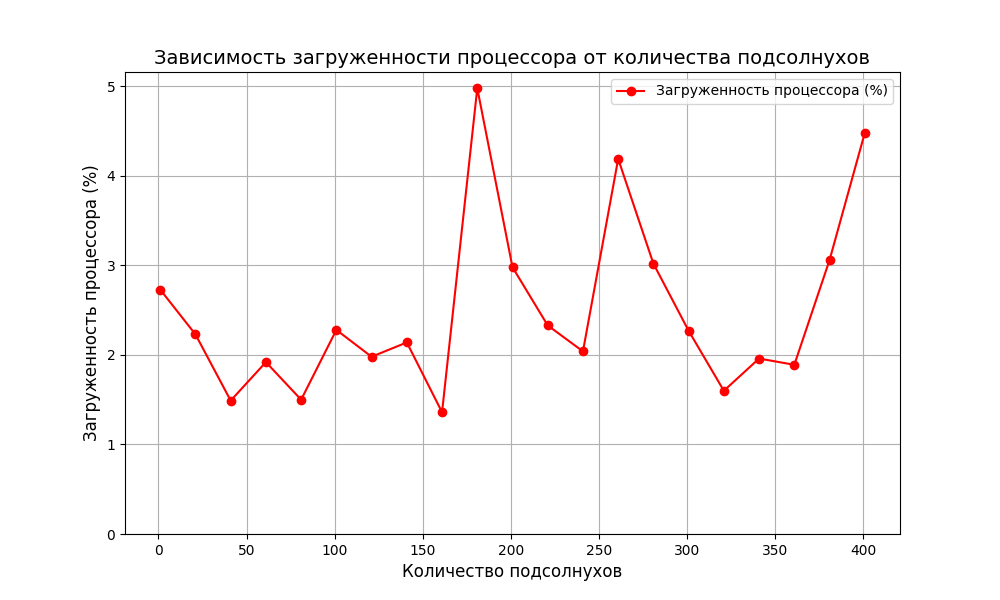
\includegraphics[width=155mm]{images/graph_2}
    \caption{График анализа загруженности процессора в зависимости от количества подсолнухов.}
    \label{images:graph_2}
\end{figure}

\subsection{Общая тенденция}
Загруженность процессора остаётся относительно низкой для большинства значений количества подсолнухов (в среднем от 1,36\% до 4,98\%). Наблюдается незначительный рост загруженности процессора при увеличении количества подсолнухов, но он не является линейным.

\subsection{Локальные колебания}
В некоторых случаях загруженность процессора может снижаться при увеличении количества подсолнухов (например, для 41 подсолнуха загруженность ниже, чем для 21). Это может быть связано с:

\begin{itemize}
    \item \textbf{Распараллеливанием:} использование многопоточности позволяет эффективно распределять нагрузку на процессор;
    \item \textbf{Кэшированием вершин:} кэширование данных, связанных с костями, снижает нагрузку на процессор.
\end{itemize}

\subsection{Стабильность загруженности процессора}
Для большинства значений количества подсолнухов загруженность процессора остаётся в диапазоне 1,36\% – 4,98\%. Это указывает на эффективность использования ресурсов процессора благодаря распараллеливанию и кэшированию.

\subsection{Вывод}
Данные показывают, что загруженность процессора остаётся низкой для большинства значений количества подсолнухов благодаря использованию распараллеливания и кэширования вершин.


\section{Вывод}
В исследовательской части курсовой работы была проведена оценка производительности программного обеспечения для моделирования поля подсолнухов. Анализ времени загрузки сцены показал, что время увеличивается с ростом количества подсолнухов, хотя могут наблюдаться локальные колебания, вызванные случайными факторами. Также было установлено, что загруженность процессора остается на низком уровне благодаря эффективному использованию многопоточности и кэшированию. 

